\chapter{Arquitectura del Sistema}

\section{Visi\'on General}

PetClinic sigue una arquitectura en capas (\textit{Layered Architecture}) con una SPA (\textit{Single Page Application}) en el frontend que se comunica con el backend mediante una API REST protegida con JWT. El backend sigue el patr\'on Controller $\rightarrow$ Service $\rightarrow$ Repository $\rightarrow$ DB, con una separaci\'on estricta de responsabilidades.

\begin{figure}[H]
    \centering
    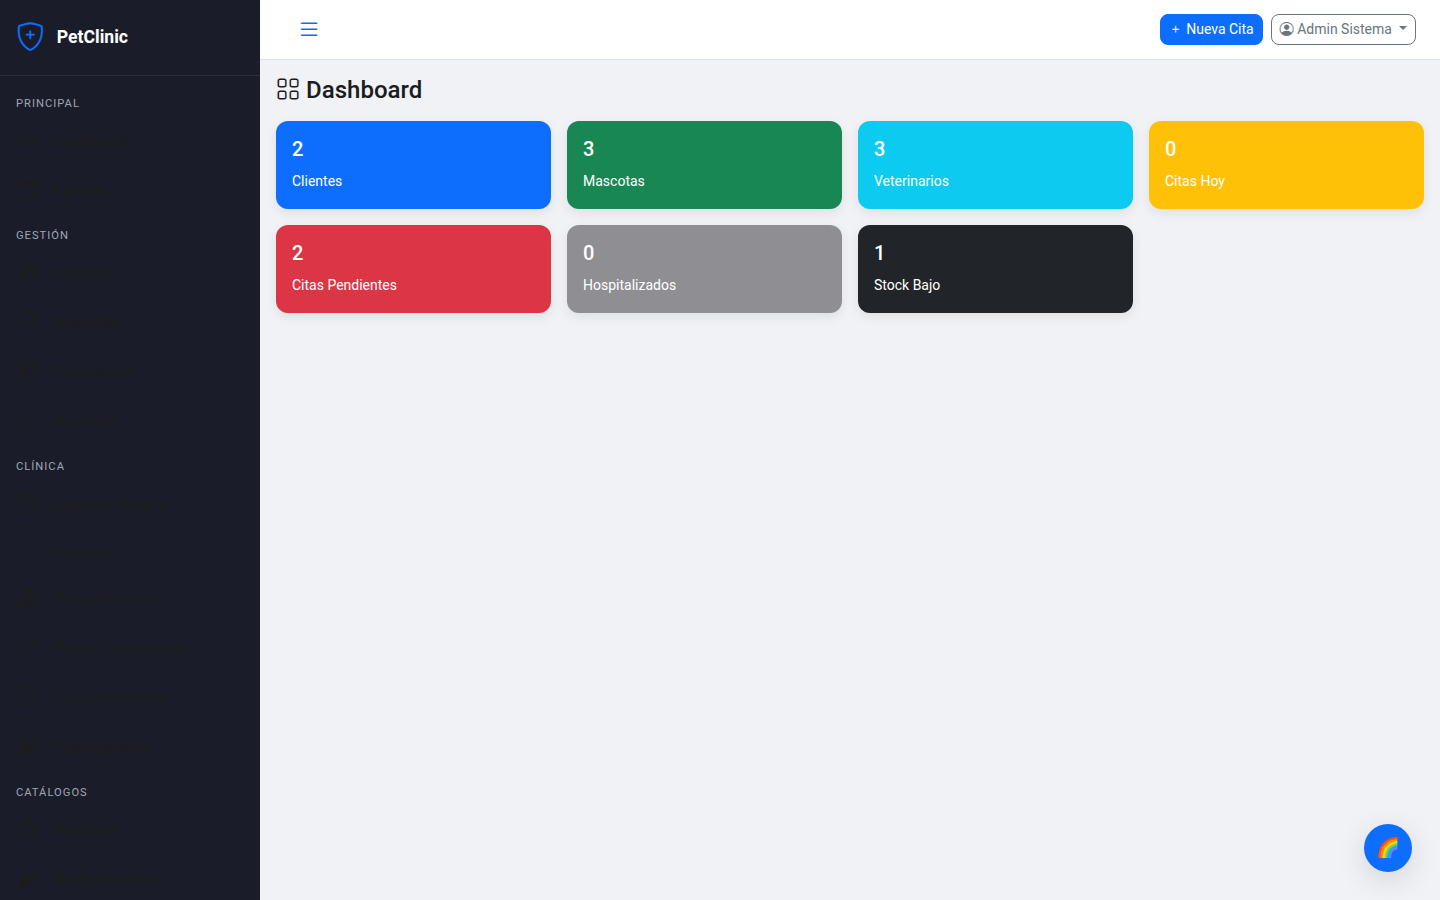
\includegraphics[width=0.9\textwidth]{images/02-dashboard}
    \caption{Pantalla principal del Dashboard de PetClinic}
    \label{fig:dashboard}
\end{figure}

\subsection{Diagrama de Capas}

\begin{verbatim}
+------------------------------------------------------------------+
|  Cliente (SPA: HTML + CSS + Vanilla JS)                           |
|  - Bootstrap 5.3 (responsive)  - FullCalendar 6.1 (agenda)       |
|  - Chart.js 4.4 (graficos)     - Bootstrap Icons                  |
+------------------------------------------------------------------+
        |  HTTP/JSON + JWT (Bearer token en header Authorization)
        v
+------------------------------------------------------------------+
|  Controller Layer (REST API)    20 controladores                  |
|  - DTO validation con Jakarta Validation                         |
|  - @RestController + @RequestMapping                             |
+------------------------------------------------------------------+
        |
        v
+------------------------------------------------------------------+
|  Service Layer (Logica de negocio)  22 servicios                  |
|  - @Transactional para operaciones atomicas                      |
|  - Inyeccion de dependencias via constructor                      |
|  - Orquestacion, calculos, reglas de negocio                      |
+------------------------------------------------------------------+
        |
        v
+------------------------------------------------------------------+
|  Repository Layer (Spring Data JPA)  19 repositorios              |
|  - JpaRepository<T, Long> con consultas derivadas                 |
|  - JPQL para consultas personalizadas                             |
|  - Paginacion y ordenamiento                                      |
+------------------------------------------------------------------+
        |
        v
+------------------------------------------------------------------+
|  Base de Datos (PostgreSQL 14+)                                   |
|  19 tablas principales + 1 tabla de auditoria                     |
+------------------------------------------------------------------+
\end{verbatim}

\section{Flujo de una Petici\'on}

Cada petici\'on HTTP atraviesa los siguientes componentes en orden:

\begin{enumerate}
    \item \textbf{JwtAuthFilter:} Extrae el token del header \texttt{Authorization: Bearer <token>}, valida la firma HMAC-SHA384, verifica expiraci\'on y extrae los claims (email, rol, userId). Si es v\'alido, establece la autenticaci\'on en el \texttt{SecurityContextHolder}.
    \item \textbf{SecurityConfig:} Verifica que el rol del usuario (ADMIN, VETERINARIO, RECEPCIONISTA, CLIENTE) tenga permiso para el endpoint solicitado mediante reglas \texttt{authorizeHttpRequests}.
    \item \textbf{Controller:} Recibe la petici\'on HTTP, valida los DTOs con \texttt{@Valid} y \texttt{jakarta.validation}, y delega la l\'ogica al servicio correspondiente.
    \item \textbf{Service:} Ejecuta la l\'ogica de negocio dentro de una transacci\'on (\texttt{@Transactional}). Realiza validaciones, c\'alculos y orquestaci\'on de operaciones.
    \item \textbf{Repository:} Interact\'ua con la base de datos mediante Spring Data JPA. Las consultas personalizadas se definen con JPQL.
    \item \textbf{GlobalExceptionHandler:} Captura cualquier excepci\'on no manejada y la formatea como una respuesta JSON est\'andar con c\'odigo HTTP apropiado.
\end{enumerate}

\section{Flujo de Notificaciones en Tiempo Real (WebSocket)}

PetClinic utiliza WebSocket con STOMP sobre SockJS para notificaciones en tiempo real de cambios en citas.

\begin{verbatim}
+--------+          +------------------+          +--------------+
| Cliente|          |  Spring Backend  |          |  Otros       |
| SPA    |          |  (CitaController)|          |  Clientes    |
+--------+          +------------------+          +--------------+
    |                     |                            |
    |  POST /api/medico/  |                            |
    |  citas (crear cita) |                            |
    |-------------------->|                            |
    |                     |                            |
    |  200 OK (cita Creada)|                           |
    |<--------------------|                            |
    |                     |                            |
    |                     |  conversionService         |
    |                     |  .broadcast("/topic/citas", |
    |                     |    citaDto)                |
    |                     |--------------------------->|
    |                     |                            |
    |  STOMP message      |                            |
    |  /topic/citas       |                            |
    |<--------------------|                            |
    |                     |                            |
\end{verbatim}

La configuraci\'on WebSocket se implementa de la siguiente manera:

\begin{lstlisting}[language=Java, caption=Configuraci\'on WebSocket]
@Configuration
@EnableWebSocketMessageBroker
public class WebSocketConfig implements WebSocketMessageBrokerConfigurer {
    @Override
    public void configureMessageBroker(MessageBrokerRegistry config) {
        config.enableSimpleBroker("/topic");
        config.setApplicationDestinationPrefixes("/app");
    }

    @Override
    public void registerStompEndpoints(StompEndpointRegistry registry) {
        registry.addEndpoint("/ws")
                .setAllowedOriginPatterns("*")
                .withSockJS();
    }
}
\end{lstlisting}

\section{Patrones de Dise\~no}

\subsection{Patrones Implementados}

\begin{longtable}{|p{4cm}|p{10cm}|}
\hline
\textbf{Patr\'on} & \textbf{Implementaci\'on} \\
\hline
Singleton & Spring Beans (\texttt{@Service}, \texttt{@Repository}, \texttt{@Controller}) \\
\hline
Inyecci\'on de Dependencias & Constructor injection en todas las clases \\
\hline
Factory & Spring Data JPA genera repositorios autom\'aticamente \\
\hline
Chain of Responsibility & Security Filter Chain (\texttt{JwtAuthFilter} $\rightarrow$ \texttt{UsernamePasswordAuthenticationFilter}) \\
\hline
Observer / Pub-Sub & WebSocket STOMP para actualizaciones de citas en tiempo real \\
\hline
Strategy & \texttt{PasswordEncoder} (BCrypt) intercambiable \\
\hline
Template Method & JPA Lifecycle Callbacks (\texttt{@PrePersist}, \texttt{@PreUpdate}) \\
\hline
DTO Pattern & \texttt{CitaDto}, \texttt{FacturaDto}, \texttt{LoginRequest/Response} separan API de entidades \\
\hline
Global Exception Handler & \texttt{@RestControllerAdvice} con \texttt{GlobalExceptionHandler} \\
\hline
CommandLineRunner & \texttt{DataInitializer} para seed data al arrancar \\
\hline
DAO Pattern & Repositorios encapsulan operaciones de base de datos \\
\hline
Scheduling & \texttt{@Scheduled} en \texttt{VacunaScheduler} para alertas autom\'aticas \\
\hline
Facade & Servicios act\'uan como fachada ante operaciones complejas (ej: \texttt{FacturaService}) \\
\hline
\end{longtable}

\section{Diagrama de Componentes}

\subsection{Capas del Sistema}

\paragraph{Capa de Presentaci\'on (Frontend)}
SPA construida con HTML, CSS y JavaScript vanilla. Utiliza Bootstrap 5 para el dise\~no responsive, FullCalendar 6 para la agenda de citas, Chart.js 4 para gr\'aficos de reportes. Se comunica con el backend mediante peticiones HTTP REST con autenticaci\'on JWT. Las actualizaciones en tiempo real llegan v\'ia WebSocket STOMP.

\paragraph{Capa de API REST (Controller)}
20 controladores REST que exponen endpoints para cada m\'odulo del sistema. Los controladores reciben y devuelven DTOs, nunca entidades JPA directamente. Utilizan \texttt{@Valid} para validaci\'on autom\'atica de entrada y \texttt{ResponseEntity} para control de c\'odigos HTTP.

\paragraph{Capa de Negocio (Service)}
22 servicios que encapsulan toda la l\'ogica de negocio. Los servicios son transaccionales y contienen validaciones, c\'alculos y orquestaci\'on de operaciones. Ejemplos: \texttt{CitaService} valida disponibilidad, \texttt{FacturaService} maneja descuento de stock, \texttt{PdfService} genera documentos.

\paragraph{Capa de Persistencia (Repository)}
19 interfaces de repositorio que extienden \texttt{JpaRepository} con consultas personalizadas mediante JPQL y m\'etodos derivados. Cada repositorio incluye consultas espec\'ificas como b\'usqueda por texto libre, agregaciones y filtros por estado.

\paragraph{Capa de Seguridad}
4 componentes de seguridad: \texttt{JwtTokenProvider} genera y valida tokens, \texttt{JwtAuthFilter} intercepta peticiones, \texttt{SecurityConfig} configura reglas de acceso, \texttt{CustomUserDetailsService} carga usuarios de la base de datos.

\section{Esquema de Navegaci\'on}

La aplicaci\'on cuenta con dos modos de navegaci\'on:

\begin{itemize}
    \item \textbf{Modo Staff (Personal):} Barra lateral con secciones para administraci\'on cl\'inica (Dashboard, Agenda, Clientes, Mascotas, Facturaci\'on, Reportes, Historial M\'edico, Vacunas, Hospitalizaci\'on, Planes, Consentimientos, Odontograma, Servicios, Medicamentos, Admin, Auditor\'ia, Configuraci\'on).
    \item \textbf{Modo Cliente:} Barra lateral simplificada con secciones personales (Inicio, Mis Mascotas, Mis Citas, Mis Facturas, Mi Perfil).
\end{itemize}
